\begin{appendices}
\chapter{Verbose Queue Length Stabilisation Results Over LS Update Intervals}
\section{Average Queue Length}
    \begin{figure}[h]
        \centering
        \begin{subfigure}[b]{0.475\textwidth}
            \centering
            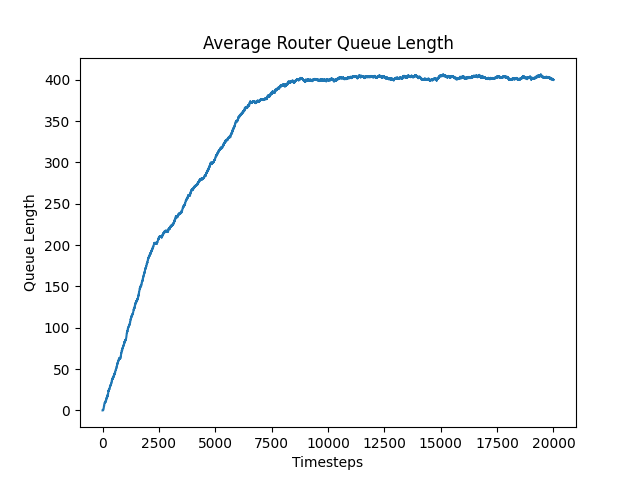
\includegraphics[width=\textwidth]{figs/appendix/average_ls=1.png}
            \caption[]{Average router queue length (LS update interval = 1)}
        \end{subfigure}
        \hfill
        \begin{subfigure}[b]{0.475\textwidth}
            \centering
            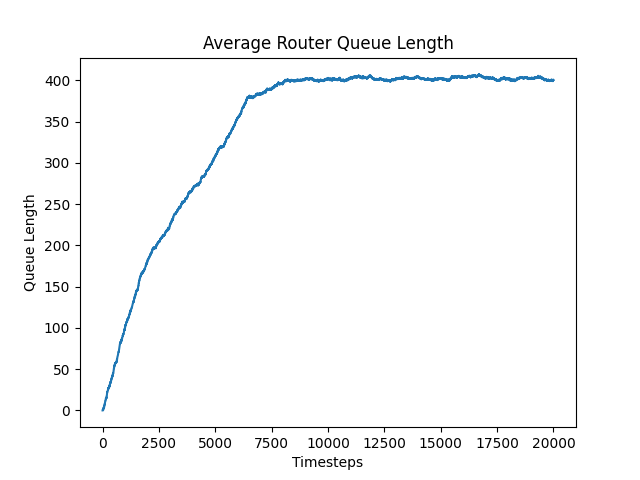
\includegraphics[width=\textwidth]{figs/appendix/average_ls=10.png}
            \caption[]{Average router queue length (LS update interval = 10)}
        \end{subfigure}
    \end{figure}
    \begin{figure}[H]\ContinuedFloat
        \centering
        \begin{subfigure}[b]{0.475\textwidth}
            \centering
            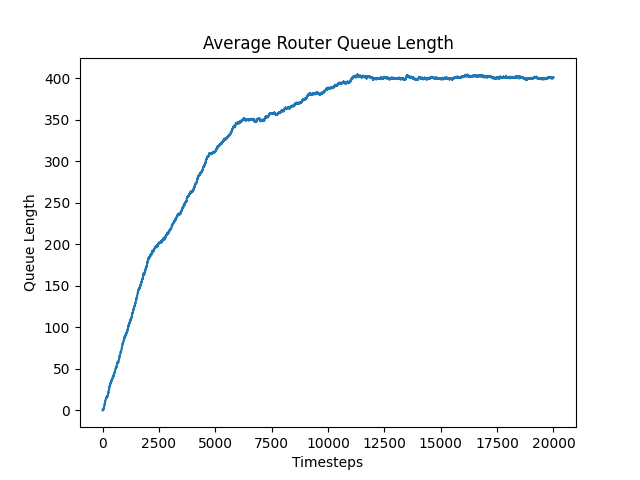
\includegraphics[width=\textwidth]{figs/appendix/average_ls=50.png}
            \caption[]{Average router queue length (LS update interval = 250)}
        \end{subfigure}
        \hfill
        \begin{subfigure}[b]{0.475\textwidth}
            \centering
            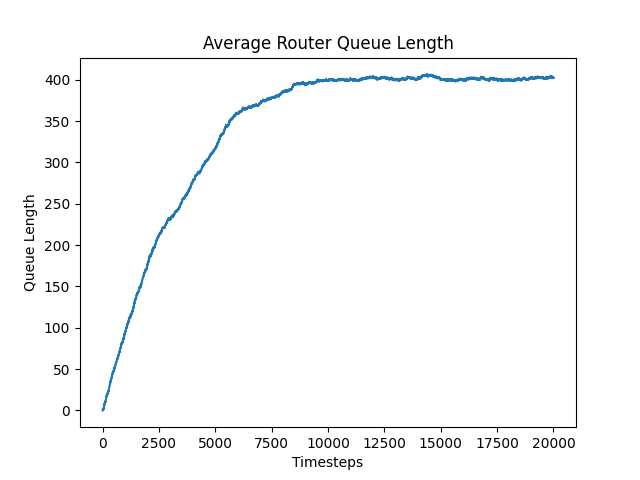
\includegraphics[width=\textwidth]{figs/appendix/average_ls=500.png}
            \caption[]{Average router queue length (LS update interval = 500)}
        \end{subfigure}
    \end{figure}
    \begin{figure}[H]\ContinuedFloat
        \centering
        \begin{subfigure}[t]{0.475\textwidth}
            \centering
            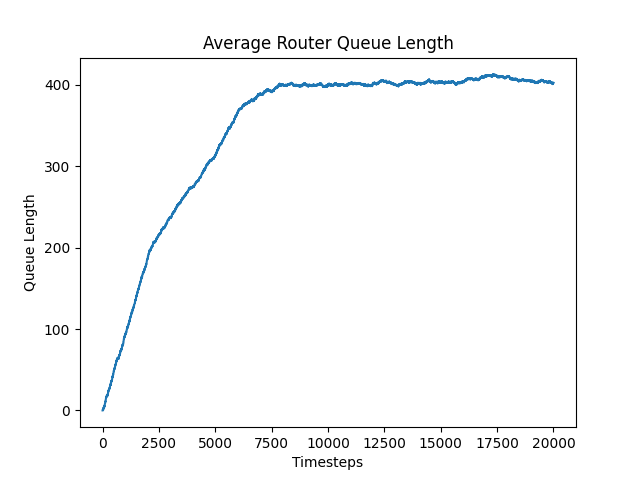
\includegraphics[width=\textwidth]{figs/appendix/average_ls=1000.png}
            \caption[]{Average router queue length (LS update interval = 1000)}
            \label{fig:avgq-1000}
        \end{subfigure}
        \hfill
        \begin{subfigure}[t]{0.475\textwidth}
            \centering
            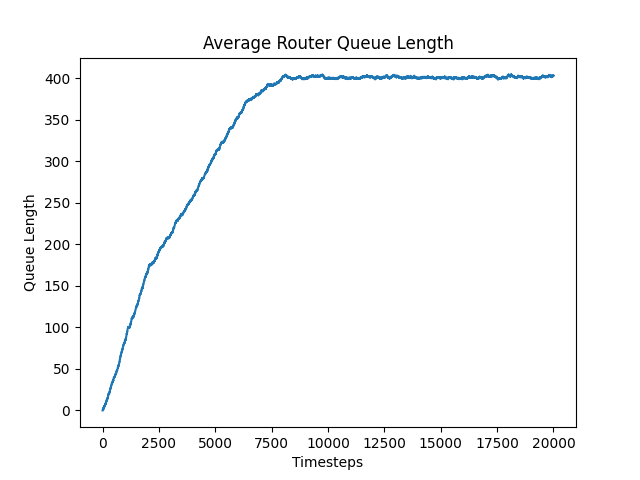
\includegraphics[width=\textwidth]{figs/appendix/average_ls=10000.png}
            \caption[]{Average router queue length (LS update interval = 10000)}
            \label{fig:avgq-10000}
        \end{subfigure}
    \end{figure}
    
\section{Variance of Queue Length}
\lfix{Trim variance graphs to same length as averages}
    \begin{figure}[H]
        \centering
        \begin{subfigure}[b]{0.475\textwidth}
            \centering
            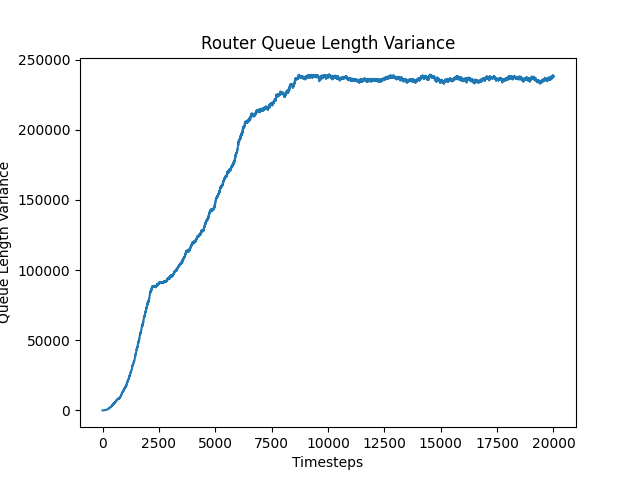
\includegraphics[width=\textwidth]{figs/appendix/variance_ls=1.png}
            \caption[]{Variance of router queue length (LS update interval = 1)}
            \label{fig:qvar-1}
        \end{subfigure}
        \hfill
        \begin{subfigure}[b]{0.475\textwidth}
            \centering
            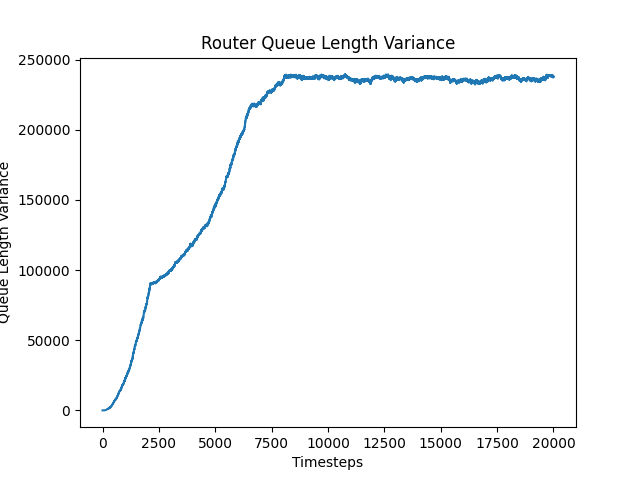
\includegraphics[width=\textwidth]{figs/appendix/variance_ls=10.png}
            \caption[]{Variance of router queue length (LS update interval = 10)}
            \label{fig:qvar-10}
        \end{subfigure}
    \end{figure}
    \begin{figure}[H]\ContinuedFloat
        \centering
        \begin{subfigure}[b]{0.475\textwidth}
            \centering
            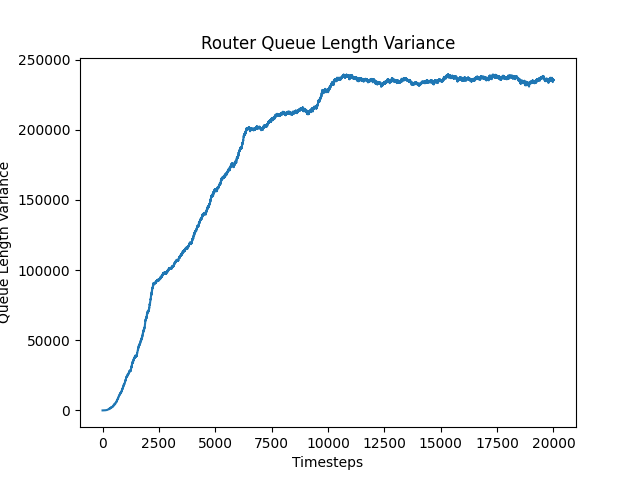
\includegraphics[width=\textwidth]{figs/appendix/variance_ls=250.png}
            \caption[]{Variance of router queue length (LS update interval = 250)}
            \label{fig:qvar-250}
        \end{subfigure}
        \hfill
        \begin{subfigure}[b]{0.475\textwidth}
            \centering
            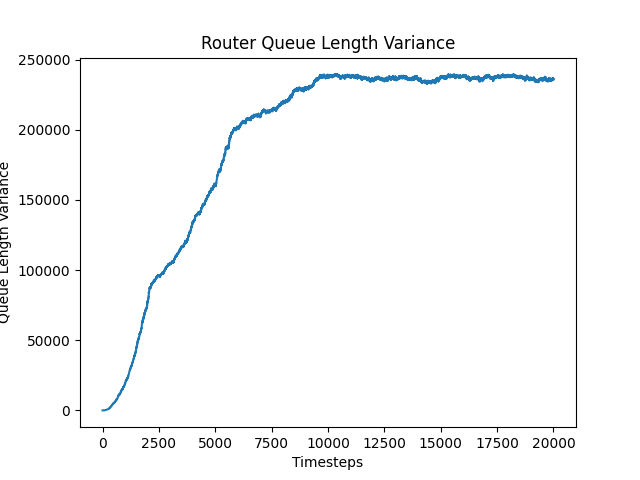
\includegraphics[width=\textwidth]{figs/appendix/variance_ls=500.png}
            \caption[]{Variance of router queue length (LS update interval = 500)}
            \label{fig:qvar-500}
        \end{subfigure}
    \end{figure}
    \begin{figure}[H]\ContinuedFloat
        \begin{subfigure}{0.475\textwidth}
            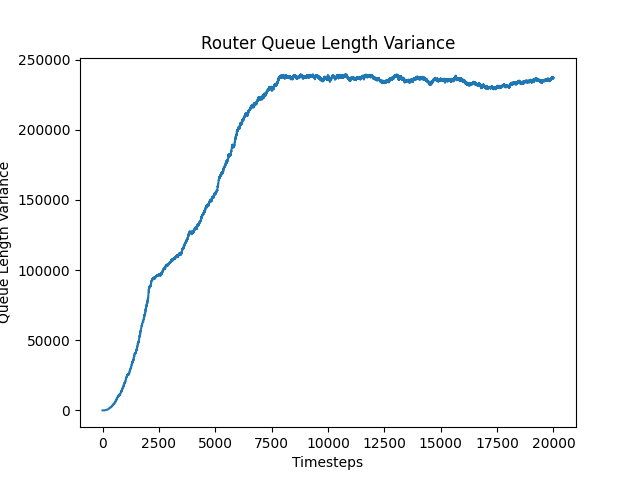
\includegraphics[width=\textwidth]{figs/appendix/variance_ls=1000.png}
            \caption[]{Variance of router queue length (LS update interval = 1000)}
            \label{fig:qvar-1000}
        \end{subfigure}
        \hfill
        \begin{subfigure}[H]{0.475\textwidth}
            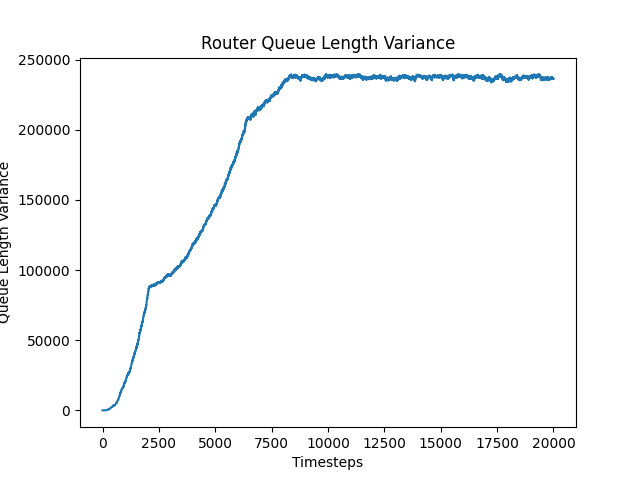
\includegraphics[width=\textwidth]{figs/appendix/variance_ls=10000.png}
            \caption[]{Variance of router queue length (LS update interval = 10000)}
            \label{fig:qvar-10000}
        \end{subfigure}
    \end{figure}
\end{appendices}
